% 第二章:导数与微分
\chapter{导数与微分}
\section{导数的定义}
\begin{example}{}{}
    已知$x,y>0$,且$x^2+9y^2=12$,则$\dfrac{x+2}{y+1}-3x$的最小值为\underline{\hspace{2cm}}.
\end{example}
\begin{solution}

\end{solution}
\begin{example}{}{}
    (单选)数列$a_{n}$各项为正整数且递增,$a_{n+2}=C_{a_{n+1}}^{a_{n}}$,则(~~~~~)

    \begin{tabular}{@{}ll@{}}
        A.$a_n<a_{n-1}+1$&B.$a_1,a_2,a_3$可能成等比数列\\
        C.$a_3a_4<a_5$&D.$a_3,a_4,a_5$可能成等比数列
    \end{tabular}
\end{example}
\begin{solution}
由于$a_n$递增,则A显然错误;下面考虑选项BD:
\[
    a_na_{n+2} = a_nC_{a_{n+1}}^{a_{n}}=a_{n+1}C_{a_{n+1}-1}^{a_{n}-1}=a_{n+1}^2\\\Rightarrow a_{n+1}=C_{a_{n+1}-1}^{a_{n}-1}
\]

当$a_n=1$时,代入表达式得到$a_{n+1}=C_{a_{n+1}-1}^{0}=1=a_n$,与数列递增矛盾;

当$a_n=2$时,代入表达式得到$a_{n+1}=C_{a_{n+1}-1}^{1}=a_{n+1}-1<a_{n+1}$,矛盾;

当$a_n>2$时,易得$a_{n+1}-1>2$,代入表达式得到
\[a_{n+1}=C_{a_{n+1}-1}^{a_{n}-1}\ge C_{a_{n+1}-1}^{2}=\dfrac{(a_{n+1}-1)(a_{n+1}-2)}{2}\]

解方程发现无整数解,而且由于$C_{a_{n+1}-1}^{1}=a_{n+1}-1$是小于$a_{n+1}$的最大整数,且有

\[C_{a_{n+1}-1}^{1}<C_{a_{n+1}-1}^{2},~~C_{a_{n+1}-1}^{2}\ne a_{n+1}\]

只可能是$C_{a_{n+1}-1}^{2}> a_{n+1}$.

雪上加霜的是,$C_{a_{n+1}-1}^{2}$和$C_{a_{n+1}-1}^{1}$中间没有数可以等于$C_{a_{n+1}-1}^{m}$,所以BD错误;

考虑C,易得$a_1\ne1,a_2\ge 4,a_3\ge6,a_4=C_{a_3}^{a_2}>2a_3+1$,由
\[a_5=C_{a_4}^{a_3}>a_3a_4 \Rightarrow a_3^2<C_{a_{4}-1}^{a_{3}-1}<C_{2a_3}^{a_3-1}\]

转化为$a_3^3+a_3<C_{2a_3}^{a_3}$这是显然成立的,故本题目选C
\end{solution}
\begin{example}{}{}
    已知$\triangle{ABC}$中,$A=3B=9C$,则$\cos A\cos B+\cos B\cos C+\cos C\cos A=$\underline{\hspace{1cm}}.
\end{example}
\begin{solution}
解得$A=\dfrac{9\pi}{13},B=\dfrac{3\pi}{13},C=\dfrac{\pi}{13}$考虑积化和差:
\begin{align*}
&\cos A\cos B+\cos B\cos C+\cos C\cos A\\
&=\dfrac12(\cos(A+B)+\cos(A-B)+\cos(B+C)+\cos(B-C)+\cos(A+C)+\cos(A+C))\\
&=\dfrac12(\cos\dfrac{12\pi}{13}+\cos\dfrac{6\pi}{13}+\cos\dfrac{4\pi}{13}+\cos\dfrac{2\pi}{13}+\cos\dfrac{10\pi}{13}+\cos\dfrac{8\pi}{13})\\
&=\dfrac{1}{2\sin\dfrac{\pi}{13}}\sin\dfrac{\pi}{13}(\cos\dfrac{2\pi}{13}+\cos\dfrac{4\pi}{13}+\cos\dfrac{6\pi}{13}+\cos\dfrac{8\pi}{13}+\cos\dfrac{10\pi}{13}+\cos\dfrac{12\pi}{13})\\
&=\dfrac{1}{4\sin\dfrac{\pi}{13}}(\sin\dfrac{\pi}{13}-\sin\dfrac{3\pi}{13}+\sin\dfrac{3\pi}{13}-\sin\dfrac{5\pi}{13}+\sin\dfrac{5\pi}{13}-\sin\dfrac{7\pi}{13}\\
&~~~~~~~~~~~~~~~~+\sin\dfrac{7\pi}{13}-\sin\dfrac{9\pi}{13}+\sin\dfrac{9\pi}{13}-\sin\dfrac{11\pi}{13}+\sin\dfrac{11\pi}{13}-\sin\dfrac{13\pi}{13})\\
&=-\dfrac14
\end{align*}
\end{solution}
\begin{theorem}{阿贝尔求和}{}
    设$B_n$是数列$b_n$的前$n$项和,当$n\ge 2$时,有:\vspace{-5pt}\[
    \sum_{i=1}^na_ib_i=a_nB_n-\sum_{i=1}^{n-1}(a_{i+1}-a_i)B_n\]
\end{theorem}
\begin{myproof}
    当$n\ge 2$时,有
    \begin{align*}
        \sum_{i=1}^na_ib_i=&a_1b_1+\sum_{i=2}^{n}a_i(B_i-B_{i-1})\\
        =&a_1b_1+\sum_{i=2}^{n}a_iB_i-\sum_{i=2}^{n}a_iB_{i-1}\\
        =&\sum_{i=1}^{n}a_iB_i-\sum_{i=1}^{n-1}a_{i+1}B_i\\
        =&a_nB_n-\sum_{i=1}^{n-1}(a_{i+1}-a_i)B_n
    \end{align*}
\end{myproof}
\begin{example}{}{}
    设数列$\{a_n\}$的各项均为实数,且当$n\ge 2$时,$a_{n+1}+a_{n-1}=|a_n|$.证明:

    (1)存在大于$1$的正整数$m$使得$a_m\le 0$

    (2)存在正整数$m$使得$a_m\le 0,~a_{m+1}\le 0$

    (3)$a_n=a_{n+9}$ 
\end{example}
% 图片插入示例(注释掉,避免报错)
% \begin{figure}[htbp]
%     \centering
%     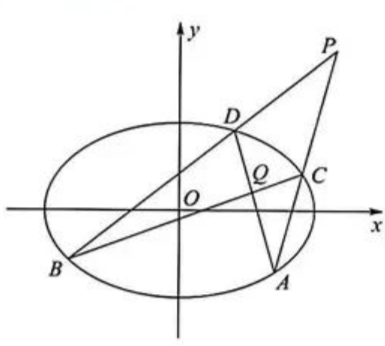
\includegraphics[width=0.6\textwidth]{flg/example.png}
%     \caption{导数的几何意义}
%     \label{fig:derivative}
% \end{figure}